\documentclass[a4paper,10pt]{report} % Wechsel von 'article' zu 'report' für Kapitelunterstützung

\usepackage{graphicx}

\usepackage[backend=biber]{biblatex}
\addbibresource{citations.bib}

\title{} % Leer lassen, da der Titel manuell gestaltet wird
\author{} % Leer lassen, da der Autor manuell gestaltet wird

\begin{document}

\begin{titlepage}
    \centering
    \vspace*{1cm}
    
    \textbf{\LARGE Optimierung eines PID-gesteuerten DC-DC-Konverters mit maschinellem Lernen}
    
    \vspace{1.5cm}
    
    \textbf{Patryk Krzyzanski}
    
    \vspace{1.5cm}
    
    Erstprüfer: Prof. Dr.-Ing. Bernhard Wicht\\
    Zweitprüfer: Dr.-Ing. Markus Olbrich
    
    \vspace{1.5cm}
    
    \textbf{Leibniz Universität Hannover}\\
    Abteilung: Institut für Mikroelektronische Systeme
    
    \vspace{1cm}
    
    \today
    
\end{titlepage}
 % Manuelle Titelseite
\begin{abstract}
In dieser Arbeit wird die Verwendung neuronaler Netze zur Optimierung und Steuerung eines PID-regulierten DC-Konverters untersucht. Das Ziel besteht darin, ein System zu entwickeln, das in der Lage ist, die altersbedingte Degradation von Schaltungskomponenten wie Kapazität und Induktivität zu überwachen und anzupassen, um die Leistung des Konverters aufrechtzuerhalten. Ein besonderer Fokus liegt auf dem Trainingsprozess und der Architektur des neuronalen Netzes. Der Trainingsprozess wird mithilfe von Methoden wie Deep Deterministic Policy Gradient (DDPG) und Bayesscher Optimierung umgesetzt. Das Training und die Schaltungssimulation werden unter Einsatz von Transientenanalyse mit SystemC durchgeführt, um eine präzise Bewertung und Auswertung der Simulationsergebnisse zu ermöglichen. Es werden Techniken zur Optimierung der Hyperparameter des neuronalen Netzes vorgestellt. Herausforderungen und Lösungsansätze im Kontext der neuronalen Netzarchitektur und des Trainings werden diskutiert. Abschließend werden die erzielten Ergebnisse und ihre Implikationen für zukünftige Forschungen präsentiert.
\end{abstract}
 % Abstract zu Beginn der Arbeit

%\tableofcontents % Inhaltsverzeichnis

%\chapter{Einleitung}
%@START In der modernen Elektrotechnik sind DC-Konverter essentiell, um Energie effizient und präzise von einer Quelle zu einem Verbraucher zu leiten.@END [Grundlagen der Elektrotechnik]
%
%@START Mit der Zeit können jedoch Schaltungskomponenten wie Kapazitäten und Induktivitäten durch verschiedene Umwelteinflüsse degradieren, was ihre Funktionsweise beeinträchtigt.@END [Studien zur Degradation von Elektronikkomponenten]
%
%@START Hier stellt sich die Frage: Wie kann man die Leistungsfähigkeit dieser Konverter trotz solcher Alterungsprozesse aufrecht erhalten?@END [Herausforderungen bei der Wartung von Elektronikkomponenten]
%
%@START Die Antwort könnte in der Anwendung von künstlichen neuronalen Netzen liegen.@END [Einführung in künstliche neuronale Netze]
%
%
%@START In dieser Arbeit wird untersucht, wie neuronale Netze dazu genutzt werden können, um die Degradation von Schaltungskomponenten zu überwachen und die PD-Koeffizienten eines DC-Konverters entsprechend anzupassen. Dabei werden Themen wie die Architektur des Netzes, Trainingsmethoden und -umgebungen, sowie die Herausforderungen beim Training und deren Lösungsansätze behandelt.@END [Spezifische Studien zur Optimierung von DC-Konvertern mit neuronalen Netzen]

\chapter{Einleitung} 
Die effiziente und präzise Lenkung von Energie von einer Quelle zu einem Verbraucher stellt eine zentrale Herausforderung in der modernen Elektrotechnik dar. Gleichspannungswandler (DC-DC Konverter) spielen hier eine entscheidende Rolle \cite[p.~70]{wensdesign2022}. Es existieren verschiedene Methoden zur DC-DC-Spannungsumwandlung, jede mit ihren spezifischen Vor- und Nachteilen, abhängig von unterschiedlichen Betriebsbedingungen und Spezifikationen \cite[p.~70]{wensdesign2022}.

Es wird zunehmend klar, dass bestimmte Schlüsselkomponenten, insbesondere Kapazitäten, eine Tendenz zur Degradation aufweisen. Diese Degradation ist häufig auf vielfältige Umwelteinflüsse zurückzuführen. Sie kann signifikante Auswirkungen auf die Funktionalität und Integrität der betroffenen Schaltungen haben. Daher ist es plausibel anzunehmen, dass die Lebensdauer und Effizienz von elektronischen Systemen erheblich beeinträchtigt werden könnten, wenn diese Degradationsmechanismen nicht sorgfältig betrachtet und adressiert werden.

Wissenschaftliche Untersuchungen stützen diese Beobachtungen. Jeong et al. haben in ihrem Artikel "Degradation-Sensitive Control Algorithm Based on Phase Optimization for Interleaved DC–DC Converters" spezifische Degradationsprozesse in DC-DC-Wandlern aufgezeigt. Dabei wurde insbesondere der äquivalente Serienwiderstand (ESR) von Kondensatoren als ein Hauptindikator für Degradation identifiziert \cite[p.~1]{jeong2023degradation}.

In einem ähnlichen Kontext haben Kulkarni et al. die systemischen Auswirkungen von Degradationen auf kritische Avioniksysteme hervorgehoben. Ihre Studien zeigen, dass solche Degradationen ernsthafte Konsequenzen für Navigationssysteme wie das Global Positioning System (GPS) und Inertial-Navigationssysteme haben können \cite[p.~3]{kulkarni_model-based_2023}.

Diese Erkenntnisse betonen die Notwendigkeit, die Mechanismen der Degradation elektronischer Komponenten auf Makro- und Mikroebene genau zu verstehen. Nur so können innovative Lösungen entwickelt werden, die solche Phänomene minimieren oder sogar verhindern können.

Ein vielversprechender Ansatz könnte in der Anwendung von künstlichen neuronalen Netzen (KNN) liegen. Wie Steven L. Brunton und J. Nathan Kutz in ihrem Werk "Data-Driven Science and Engineering: Machine Learning, Dynamical Systems, and Control" darlegen, bieten KNN ausgezeichnete Möglichkeiten zur Steuerung komplexer, nichtlinearer Systeme, einschließlich elektronischer Schaltungen \cite[p.~270]{brunton2019data}. Almawlawe et al. konnten in ihrer Studie zeigen, dass neuronale Netzwerk-Controller im Vergleich zu traditionellen Proportional-Integral-Derivative (PID)- und digitalen Gleitmodus-Reglern eine überlegene Leistung bei der Ausgangsspannungsverfolgung eines Buck DC/DC-Konverters bieten \cite[p.~8]{Almawlawe2023}. Miguel Morales betont in "Grokking Deep Reinforcement Learning", dass KNN einer der leistungsfähigsten Funktionsapproximatoren sind und oft andere Methoden übertreffen \cite[p.~22]{morales2020grokking}.

In dieser Arbeit wird untersucht, wie KNN dazu genutzt werden können, um die Degradation von Schaltungskomponenten zu überwachen und die PID-Koeffizienten eines DC-Konverters entsprechend anzupassen. Themen wie die Architektur des Netzes, Trainingsmethoden und -umgebungen, sowie Herausforderungen beim Training und deren Lösungsansätze werden behandelt.

\chapter{Grundlagen}




\textbf{Einleitung zum Kapitel}

Dieses Kapitel dient als umfassende Grundlage für die Erforschung der Rolle neuronaler Netze in der Optimierung und Steuerung von PID-regulierten DC-Konvertern. Im Fokus stehen sowohl die Grundlagen der DC-DC-Konvertertechnologie als auch spezielle Herausforderungen, die in diesem Kontext auftreten können, wie beispielsweise die altersbedingte Degradation von Schaltungskomponenten. Darüber hinaus bietet das Kapitel einen Überblick über moderne Optimierungsmethoden wie DDPG (Deep Deterministic Policy Gradients) und Bayessche Optimierung, die in der aktuellen Forschung Bedeutung erlangt haben.

Der Inhalt dieses Kapitels zielt darauf ab, den Leser umfassend auf die Herausforderungen, technischen Lösungen und innovativen Ansätze in diesem sich schnell entwickelnden Forschungsfeld vorzubereiten.

%1. Gleichspannungswandler (DC-DC-Konverter)


\section{Elektrotechnik}
\subsection{Buck-Konverters}

\paragraph{Hauptkomponenten und Funktionen eines DC-DC-Konverters}

Die Wandlung von Gleichspannung (DC) in eine andere Gleichspannung ist ein kritischer Aspekt in der Elektronik und Energieversorgung. Ein weit verbreitetes Schaltungsdesign, das diese Funktion ausführt, ist der Buck-Konverter. In der Literatur wird dieser als eine Standardmethode für DC-DC-Wandlung beschrieben \cite[p.~66]{wensdesign2022}.



\paragraph{MOSFET-Transistor}
Der MOSFET-Transistor agiert als elektronischer Schalter, der den Stromfluss in der Schaltung reguliert. Im Vergleich zu alternativen Schaltelementen bietet der MOSFET eine signifikante Effizienzsteigerung durch minimale Leistungsverluste. Dies wird durch Phänomene wie Trägermobilität und die damit verbundene Widerstandsfähigkeit gegenüber thermischen Ausfällen ermöglicht \cite[p.~29]{choi2013pulsewidth}.

\paragraph{Induktivität (Spule)}
Die Induktivität dient der temporären Energiespeicherung in Form eines magnetischen Feldes, das beim Stromfluss durch die Spule generiert wird. Dies ist insbesondere relevant in Anwendungen wie Solenoid-Antriebsschaltungen, wo die Induktivität als Energiespeicher und -überträger fungiert \cite[p.~54]{choi2013pulsewidth}.

\paragraph{Diode}
Die Diode ist so ausgerichtet, dass sie den Strom nur in einer Richtung passieren lässt. Dies ist insbesondere wichtig, wenn der MOSFET-Transistor deaktiviert ist. Als passive Schalter werden oftmals schnelle Erholungsdioden oder Schottky-Dioden aufgrund ihrer exzellenten Schalteigenschaften verwendet \cite[p.~29]{choi2013pulsewidth}.

\paragraph{Kondensator}
Der Kondensator dient der Glättung der Ausgangsspannung und speichert Energie für die Last. Er spielt eine wichtige Rolle in der Dynamik der Schaltung und ermöglicht eine stabilere Energieversorgung \cite[p.~54]{Kularatna2012}.
\paragraph{Regelung und Anwendungen}

In der Praxis werden Buck-Konverter oft von einer nicht-idealen Spannungsquelle gespeist und müssen daher unter variablen Eingangsspannungen und Lastströmen arbeiten \cite[p.~124,120,113]{choi2013pulsewidth}.. Daher ist eine geschlossene Regelungsschleife erforderlich, um eine konstante Ausgangsspannung sicherzustellen.

Buck-Konverter finden eine breite Anwendung in verschiedenen elektronischen Geräten und Systemen. Ihr hoher Wirkungsgrad, der in der Regel zwischen 75\% und 98\% liegt, macht sie besonders attraktiv.


\begin{figure}[htbp]
    \centering
    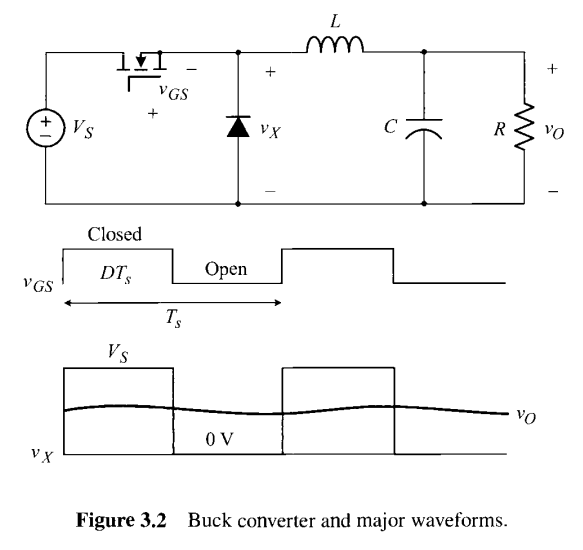
\includegraphics[width=0.4\linewidth]{2Grundlagen/111DCDC.png}
    \caption{Schematische Darstellung eines DC-DC Konverters. Quelle: \cite[Seite 88]{choi2013pulsewidth}}
    \label{fig:dcdc_converter}
\end{figure}




\subsection{Degradation von Kondensatoren und MOSFETs in DC-DC-Konvertern}

Die Zuverlässigkeit und Effizienz von DC-DC-Konvertern sind zunehmend von der Degradation ihrer Schlüsselkomponenten, insbesondere von Kondensatoren und MOSFETs, beeinträchtigt.

\paragraph{Kondensatoren}

Kondensatoren sind anfällig für verschiedene Arten von Ausfallmodi, darunter Änderungen des Verlustfaktors (tan $\delta$), der Impedanz und des Dissipationsfaktors. Diese Parameter sind entscheidend für die Beurteilung der Zuverlässigkeit eines Systems. Ebenso ist die erhöhte Äquivalente Serienresistenz (ESR) von Elektrolytkondensatoren, die elektrischen und thermischen Belastungen ausgesetzt sind, ein weiterer entscheidender Faktor für die Degradation.\cite[pp. 1]{jeong2023degradation}

\paragraph{MOSFETs}

Bei MOSFETs kann die Degradation aufgrund von thermischen Spannungen zu einem Gate-Source-Kurzschluss oder einem Drain-Source-Kurzschluss führen\. Die Degradation der Transistoren erhöht deren Leistungsverluste und beschleunigt damit den Degradationsprozess weiter.\cite[pp. 190]{wensdesign2022}



\paragraph{Kontrolle und Überwachung}

Aktuelle Forschungsbemühungen konzentrieren sich auf die Entwicklung von Kontrollalgorithmen, um die Degradation zu verzögern und die Zuverlässigkeit der Konverter zu erhöhen. Dazu gehören auch Verfahren zur Schätzung des Zustands der Degradation in Echtzeit.
\cite[p.~24, p.~310-311]{choi2013pulsewidth}

\paragraph{Integration mit neuronalen Netzen für Kondensatoren und MOSFETs}

Neuronale Netze können verwendet werden, um aktiv entgegensteuernde Maßnahmen zur Verlangsamung der Degradation von Schlüsselkomponenten wie Kondensatoren und MOSFETs in DC-DC-Konvertern einzuleiten. Durch die kontinuierliche Analyse von Betriebsparametern wie Temperatur und Spannung sind diese Netze in der Lage, den Zustand der Degradation in Echtzeit zu erfassen. Sobald kritische Zustände erkannt werden, können die neuronalen Netze automatisch die PID-Koeffizienten des Konverters anpassen, um die Degradation zu minimieren und die Zuverlässigkeit des Systems zu erhöhen.
\cite[p.~22]{morales2020grokking}

\subsection{PID-Regler}
Der PID-Regler (Proportional-Integral-Derivativ) ist eine weit verbreitete Regelungsstrategie in industriellen Steuerungssystemen und verschiedenen Arten von Anwendungen. Er ist unerlässlich für die Regelung von Prozessen wie Geschwindigkeit, Temperatur und Spannung~\cite[p.~2]{Hussein2011PIDGA}.

\paragraph{Proportionalanteil (P)}
Diese Komponente erzeugt einen Ausgangswert, der proportional zum aktuellen Fehlerwert ist. Die proportionale Reaktion kann durch Multiplikation des Fehlers mit einer Konstanten namens \( K_p \) eingestellt werden, die als Proportionalverstärkung bezeichnet wird.
\begin{equation}
P_{\text{out}} = K_p \times e(t)
\end{equation}

\paragraph{Integralanteil (I)}
Diese Komponente befasst sich mit der Akkumulation vergangener Fehler. Wenn der Fehler über einen längeren Zeitraum vorhanden war, wird er akkumuliert (Integral des Fehlers), und der Regler wird den Steuerausgang in Beziehung zu einer Konstanten \( K_i \) ändern, die als Integralverstärkung bekannt ist.
\begin{equation}
I_{\text{out}} = K_i \times \int e(t) \, dt
\end{equation}

\paragraph{Differentiantanteil (D)}
Diese Komponente liefert einen Steuerausgang, um die Änderungsrate des Fehlers zu kompensieren. Der Beitrag des Differenzierungsanteils zur gesamten Steueraktion wird als Differenzierungsverstärkung \( K_d \) bezeichnet.
\begin{equation}
D_{\text{out}} = K_d \times \frac{d}{dt} e(t)
\end{equation}
\cite[p.~1744]{russell2021ai}

\paragraph{Die PID-Regelungsgleichung}
Die PID-Regelungsgleichung kombiniert diese drei Komponenten, um den Steuerausgang zu erzeugen:
\begin{equation}
\text{Steuerausgang} = P_{\text{out}} + I_{\text{out}} + D_{\text{out}}
\end{equation}
\begin{equation}
\text{Steuerausgang} = (K_p \times e(t)) + (K_i \times \int e(t) \, dt) + (K_d \times \frac{d}{dt} e(t))
\end{equation}

\paragraph{Einstellung der Verstärkungsfaktoren}
Die Konstanten \( K_p, K_i, \) und \( K_d \) werden eingestellt, um die optimale Systemleistung zu erreichen; ein schlecht eingestellter PID-Regler kann instabil, langsam oder schwingend sein.

\paragraph{Anwendungen bei Gleichstrom-Gleichstrom-Wandlern}
Im Kontext von Gleichstrom-Gleichstrom-Wandlern können PID-Regler helfen, die Ausgangsspannung zu stabilisieren, indem sie die Ausgangsspannung kontinuierlich mit der gewünschten Spannung vergleichen und handeln, um den Fehler durch Anpassung des Tastverhältnisses des Schaltelements zu minimieren~\cite[p.~4]{Almawlawe2023}.

\paragraph{Fazit}
Der PID-Regler ist eine vielseitige und weit verbreitete Regelungsstrategie. Seine Anpassungsfähigkeit und Effizienz machen ihn ideal für eine breite Palette von Anwendungen, von industriellen Prozessen bis zu modernen Technologiesystemen. Für eine erweiterte Diskussion über verschiedene Varianten von PID-Reglern, wie zum Beispiel den Fuzzy PID-Controller, könnten Sie das Paper "Shi2020AdaptiveController" verwenden~\cite[p.~9]{Shi2020AdaptiveController}.



\subsection{Pulsweitenmodulation und ihre Darstellung}
\label{sec:PWM_Grundlagen}
Pulsweitenmodulation (PWM) ist eine Schlüsseltechnik in DC-DC-Wandlern, die zur Steuerung der Schaltkomponenten eingesetzt wird, um die Ausgangsspannung oder den Ausgangsstrom zu regulieren. Sie ermöglicht eine präzise Kontrolle, indem sie die 'Einschaltzeit' des Schalters im Vergleich zur gesamten Zykluszeit (Einschaltzeit + Ausschaltzeit) variiert.\cite{peddapelli2017pulse}

\paragraph{Tastverhältnis \(D\)}
Die Einschaltzeit ist die Zeit, der Schalter eingeschaltet ist. Das Tastverhältnis \( D \) wird mathematisch als das Verhältnis der Einschaltzeit zur gesamten Zykluszeit beschrieben:
\begin{equation}
D = \frac{\text{Einschaltzeit}}{\text{Einschaltzeit} + \text{Ausschaltzeit}}
\end{equation}

\paragraph{Proportionalanteil (P)}
Das Tastverhältnis spielt eine wichtige Rolle, da es den Mittelwert der Ausgangsspannung oder des Ausgangsstroms bestimmt. Bei der PWM wird ein Steuersignal mit einem hochfrequenten Trägersignal verglichen, um die 'Ein'- und 'Aus'-Zustände des Schalters festzulegen. Das Steuersignal stammt oft von höheren Regelkreisen wie PID-Reglern, die den Fehler zwischen Soll- und Istwert minimieren sollen.

Die Hauptmotivation für die Verwendung von PWM in Steuerungssystemen ist die Anpassung des Mittelwerts der Ausgabe an ein Referenzsignal. Zusätzlich wird versucht, harmonische Verzerrungen und Schaltverluste zu minimieren \cite{peddapelli2017pulse}.

In der Abbildung \ref{fig:PWM_converter} ist eine typische PWM-Schaltung dargestellt. Der PWM-Block und die Spannungsrückführungsschaltung im DC-DC-Wandler arbeiten zusammen, um sicherzustellen, dass die Ausgangsspannung der Referenzspannung folgt. Hierbei wird ein Steuersignal \(v_{\text{con}}\) und ein Rampensignal \(V_{\text{ramp}}\) verwendet, um die Impulsbreite des aktiven Schalters zu modulieren. Das rechte Diagramm (b) zeigt die Steuersignale und ihre Relation zueinander, wodurch das Schaltverhalten des Wandlers beeinflusst wird \cite{choi2013pulsewidth}.



\begin{figure}[htbp]
    \centering
    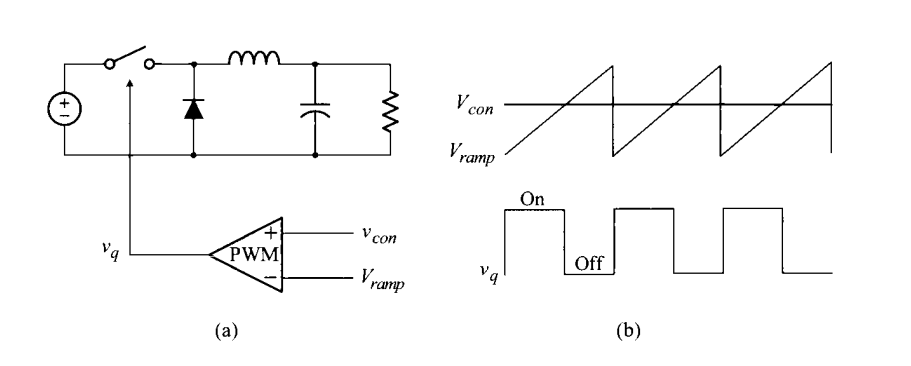
\includegraphics[width=0.8\linewidth]{2Grundlagen/141PWM.png}
    \caption{Schematische Darstellung eines PWM-Modulator. Quelle: \cite{choi2013pulsewidth}}
    \label{fig:PWM_converter}
\end{figure}


\section{Informationstechnologie}

\subsection{Einführung in Neuronale Netzwerke}
Neuronale Netzwerke bilden das rechnerische Grundgerüst für eine Vielzahl von Aufgaben in den Berei-chen maschinelles Lernen und künstliche Intelligenz. Sie sind von dem komplexen Netzwerk an Neuronen im menschlichen Gehirn inspiriert und versuchen, biologische Lernprozesse nachzuahmen \cite{aggarwal_neural_networks_2018}. In diesem Zusammenhang bieten sie ein robustes und flexibles Rahmenwerk zur Lösung komplexer Herausforderungen \cite{Goodfellow-et-al-2016}.

\subsubsection{Vorteile von Neuronalen Netzwerken}
Neuronale Netzwerke bieten mehrere entscheidende Vorteile, die ihren Einsatz in unterschiedlichen Anwendungsbereichen attraktiv machen:
\begin{itemize}
    \item \textbf{Parallelität:} Sie sind für die parallele Verarbeitung konzipiert und ermöglichen daher schnelle Berechnungen sowie Echtzeitverarbeitung.
    \item \textbf{Nichtlineare Funktionsapproximation:} Die Netzwerke sind besonders gut geeignet, nichtlineare Funktionen zu approximieren \cite{Goodfellow-et-al-2016}, was sie vielseitig einsetzbar macht.
    \item \textbf{Modellgeneralisierung:} Neuronale Netzwerke können aus einer begrenzten Datenmenge gene-ralisieren und somit präzise Vorhersagen für unbekannte Eingaben treffen.
\end{itemize}
Diese Vorteile bilden die Grundlage für ihre breite Anwendbarkeit, die im nächsten Abschnitt erläutert wird.

\subsubsection{Unterschied zwischen Biologischen und Künstlichen Neuronalen Netzwerken}
Künstliche neuronale Netzwerke bestehen aus rechnerischen Einheiten, den sogenannten Neuronen. Diese sind durch anpassbare Gewichtungen verbunden, die der Stärke synaptischer Verbindungen in biologischen Systemen ähneln. Lernen erfolgt durch die Anpassung dieser Gewichtungen, ähnlich wie sich die Stärken synaptischer Verbindungen in biologischen Systemen als Reaktion auf Reize ändern \cite{aggarwal_neural_networks_2018}.

\subsubsection{Deep Learning als Spezialisierung}
Deep Learning stellt einen spezialisierten Unterbereich des maschinellen Lernens dar, der neuronale Netzwerke mit drei oder mehr Schichten verwendet. Diese tiefen Netzwerke führen eine hierarchische Merkmalsextraktion durch, die es ihnen ermöglicht, immer komplexere Muster und Merkmale zu erkennen, während die Daten durch die Schichten fließen.

\subsubsection{Zusammenfassung und Ausblick}
Zusammenfassend bieten neuronale Netzwerke ein leistungsfähiges Rahmenwerk für eine Vielzahl von Aufgaben, von einfacher Mustererkennung bis hin zu komplexen Entscheidungsfindungsprozessen. Der Einsatz von mehrschichtigen Architekturen und nichtlinearen Aktivierungsfunktionen erweitert die Fähig-keiten traditioneller maschineller Lernalgorithmen \cite{aggarwal_neural_networks_2018}.

Mit dieser Grundlage werden die folgenden Abschnitte einen vertieften Einblick in die mathematischen Aspekte von neuronalen Netzwerken bieten. Insbesondere werden wir uns darauf konzentrieren, wie neuronale Netzwerke bei der Optimierung und Steuerung von PID-regulierten DC-Konvertern Anwendung finden. Dabei liegt der Fokus auf der Berücksichtigung von Alterungsprozessen und Abnutzung von Schaltungselementen wie Kapazitäten und Induktivitäten und wie diese Einflüsse mathematisch modelliert und optimiert werden können.

\subsection{Vorwärtspropagation in Neuronalen Netzwerken}
\subsubsection{Schicht-für-Schicht-Propagation}
Beginnend mit der Eingabeschicht \( A^{[0]} \), die im Wesentlichen die Eingabedaten \( X \) sind, berechnet jede nachfolgende Schicht \( Z^{[l]} \) und \( A^{[l]} \) entsprechend den oben genannten Gleichungen. Dies bildet das Kernstück der Vorwärtspropagation.

\subsubsection{Dimensionalität und Netzwerkarchitektur}
Die Anzahl der Neuronen in jeder Schicht und die Art der verwendeten Aktivierungsfunktion können die Leistung des Netzwerks erheblich beeinflussen. Es ist wichtig, die Dimensionalität jeder Schicht während der Entwurfsphase zu berücksichtigen, um ein effektives Lernen sicherzustellen.

Die Vorwärtspropagation ist ein wesentlicher Prozess in neuronalen Netzwerken, der die Übertragung von Eingabedaten durch die Netzwerkarchitektur ermöglicht, um die Ausgabe zu erzeugen \cite[p.~1421]{russell2021ai}. Sie ist eine Abfolge von mathematischen Operationen, die Gewichtungen, Biases und Aktivierungsfunktionen involvieren \cite[p.~73]{Chollet2021}.

\subsubsection{Gewichtsmatrix \( W^{[l]} \) und Bias-Vektor \( b^{[l]} \)}
Die Gewichtsmatrix für die Schicht \( l \) wird als \( W^{[l]} \) bezeichnet, und \( b^{[l]} \) ist der Bias-Vektor für dieselbe Schicht \cite[p.~46]{heaton_2012}. Diese Parameter werden während des Backpropagation-Prozesses trainiert, um den Fehler zwischen der vorhergesagten und der tatsächlichen Ausgabe zu minimieren \cite[p.~41]{aggarwal_neural_networks_2018}.

\begin{equation}
Z^{[l]} = W^{[l]} A^{[l-1]} + b^{[l]}
\end{equation}

\subsubsection{Aktivierungsfunktionen}
Eine Aktivierungsfunktion, normalerweise durch \( \sigma \) bezeichnet, transformiert die gewichtete Summe \( Z^{[l]} \) in die aktivierte Ausgabe \( A^{[l]} \) \cite[p.~1421]{russell2021ai}.

\begin{equation}
A^{[l]} = \sigma(Z^{[l]})
\end{equation}

\begin{equation}
A^{[l]} = \sigma \left( 
\begin{pmatrix}
w_{1,1}^{[l-1,l]} & w_{1,2}^{[l-1,l]} & \cdots & w_{1,m}^{[l-1,l]} \\
w_{2,1}^{[l-1,l]} & w_{2,2}^{[l-1,l]} & \cdots & w_{2,m}^{[l-1,l]} \\
\vdots & \vdots & \ddots & \vdots \\
w_{n,1}^{[l-1,l]} & w_{n,2}^{[l-1,l]} & \cdots & w_{n,m}^{[l-1,l]}
\end{pmatrix}
\begin{pmatrix}
A_1^{[l-1]} \\
A_2^{[l-1]} \\
\vdots \\
A_m^{[l-1]}
\end{pmatrix}
+
\begin{pmatrix}
b_1^{[l]} \\
b_2^{[l]} \\
\vdots \\
b_n^{[l]}
\end{pmatrix}
\right)
\end{equation}

\subsubsection{Schicht-für-Schicht-Propagation}
Beginnend mit der Eingabeschicht \( A^{[0]} \), die im Wesentlichen die Eingabedaten \( X \) sind, berechnet jede nachfolgende Schicht \( Z^{[l]} \) und \( A^{[l]} \) entsprechend den oben genannten Gleichungen \cite[p.~1421]{russell2021ai}.

\subsubsection{Dimensionalität und Netzwerkarchitektur}
Die Anzahl der Neuronen in jeder Schicht und die Art der verwendeten Aktivierungsfunktion können die Leistung des Netzwerks erheblich beeinflussen \cite[p.~1408]{russell2021ai}. Es ist wichtig, die Dimensionalität jeder Schicht während der Entwurfsphase zu berücksichtigen, um ein effektives Lernen sicherzustellen \cite[p.~73]{Chollet2021}.


\subsection{Gradientenberechnung}

Sie haben eine Kostenfunktion \( C_0 \) definiert als:
\begin{equation}
C_0 = \sum_{j=0}^{n_{L-1}} (a_j^{[L]} - y_j)^2
\end{equation}

Um die Kostenfunktion zu minimieren, müssen Sie den Gradienten in Bezug auf alle Gewichtungen und Bias berechnen. Mit Hilfe der Kettenregel können Sie die partielle Ableitung der Kostenfunktion in Bezug auf jedes Gewicht wie folgt ausdrücken:

\begin{equation}
\frac{\partial C_0}{\partial w_{jk}^{[L]}} = \frac{\partial w_{jk}^{[L]}}{\partial z_j^{[L]}} \frac{\partial z_j^{[L]}}{\partial a_j^{[L]}} \frac{\partial a_j^{[L]}}{\partial C_0}
\end{equation}

Wenn Sie den Nabla-Operator verwenden, um den Gradienten der Kostenfunktion in Bezug auf alle Gewichtungen in der Matrixform darzustellen, erhalten Sie:

\begin{equation}
\nabla_{W^{[L]}} C_0 = \begin{pmatrix}
\frac{\partial C_0}{\partial w_{11}^{[L]}} & \frac{\partial C_0}{\partial w_{12}^{[L]}} & \cdots & \frac{\partial C_0}{\partial w_{1m}^{[L]}} \\
\frac{\partial C_0}{\partial w_{21}^{[L]}} & \frac{\partial C_0}{\partial w_{22}^{[L]}} & \cdots & \frac{\partial C_0}{\partial w_{2m}^{[L]}} \\
\vdots & \vdots & \ddots & \vdots \\
\frac{\partial C_0}{\partial w_{n1}^{[L]}} & \frac{\partial C_0}{\partial w_{n2}^{[L]}} & \cdots & \frac{\partial C_0}{\partial w_{nm}^{[L]}}
\end{pmatrix}
\end{equation}

Dabei ist \( \nabla_{W^{[L]}} C_0 \) die Matrix der partiellen Ableitungen der Kostenfunktion \( C_0 \) in Bezug auf jede Gewichtung in \( W^{[L]} \).



\subsection{Rückpropagation in Neuronalen Netzwerken}

Für die Rückpropagation definieren wir den Fehler in der Ausgabeschicht durch:
\[
\frac{\partial C_0}{\partial a_j^{[L]}} = 2 \left( a_j^{[L]} - y_j \right)
\]
wobei \( a_j^{[L]} \) die Aktivierung der \( j \)-ten Einheit in der Ausgabeschicht und \( y_j \) der tatsächliche Wert für diese Einheit ist.

\paragraph{Fehler Rückpropagieren}

Der nächste Schritt besteht darin, den Fehler durch das Netzwerk zurückzupropagieren. Um den Beitrag jeder Gewichtung und jedes Bias zur Gesamtkostenfunktion zu ermitteln, berechnen wir die Ableitung der Aktivierungsfunktion \( a_j^{[L]} \) in Bezug auf die lineare Kombination \( z_j^{[L]} \):
\[
\frac{\partial z_j^{[L]}}{\partial a_j^{[L]}} = \sigma' \left( z_j^{[L]} \right)
\]
wobei \( \sigma' \left( z_j^{[L]} \right) \) die Ableitung der Aktivierungsfunktion ist.

Um die Ableitung der linearen Kombination \( z_j^{[L]} \) in Bezug auf die Gewichtung \( w_{jk}^{[L]} \) zu berechnen, verwenden wir:
\[
\frac{\partial z_j^{[L]}}{\partial w_{jk}^{[L]}} = a_k^{[L-1]}
\]

\paragraph{Kettenregel Anwenden}

Jetzt kombinieren wir alle diese Teile mit der Kettenregel:
\[
\frac{\partial C_0}{\partial w_{jk}^{[L]}} = 2 \left( a_j^{[L]} - y_j \right) \cdot \sigma' \left( z_j^{[L]} \right) \cdot a_k^{[L-1]}
\]

\paragraph{Gradienten der Kostenfunktion}

Schließlich, um den Gradienten der Kostenfunktion \( C_0 \) in Bezug auf alle Gewichtungen darzustellen, verwenden wir:
\[
\nabla W^{[L]} C_0 = \left( 2 \left( a^{[L]} - y \right) \odot \sigma' \left( Z^{[L]} \right) \right) A^{[L-1]T}
\]

Mit diesen Gradienten können Sie die Gewichtungen und Biasse im neuronalen Netzwerk aktualisieren, indem Sie einen Optimierungsansatz wie den Gradientenabstieg verwenden.

\subsection{Backpropagation im Training neuronaler Netze}

\subsubsection{Mathematische Grundlagen}

Die Gradientenmatrix für die Gewichtungen in Bezug auf die Kostenfunktion \( C_0 \) unter Verwendung des Nabla-Operators kann in der Matrixform dargestellt werden:

Dabei setzt sich jede Komponente der Matrix wie folgt zusammen:

\[
\frac{\partial C_0}{\partial w_{ij}^{[L]}} = 2(a_i^{[L]} - y_i) \cdot \sigma' (z_i^{[L]}) \cdot a_j^{[L-1]}
\]

So erhalten wir die gesamte Matrix der partiellen Ableitungen:

\[
\nabla_{W^{[L]}} C_0 = 
\begin{pmatrix}
2(a_1^{[L]} - y_1) \cdot \sigma' (z_1^{[L]}) \cdot a_1^{[L-1]} & \cdots & 2(a_1^{[L]} - y_1) \cdot \sigma' (z_1^{[L]}) \cdot a_m^{[L-1]} \\
2(a_2^{[L]} - y_2) \cdot \sigma' (z_2^{[L]}) \cdot a_1^{[L-1]} & \cdots & 2(a_2^{[L]} - y_2) \cdot \sigma' (z_2^{[L]}) \cdot a_m^{[L-1]} \\
\vdots & \ddots & \vdots \\
2(a_n^{[L]} - y_n) \cdot \sigma' (z_n^{[L]}) \cdot a_1^{[L-1]} & \cdots & 2(a_n^{[L]} - y_n) \cdot \sigma' (z_n^{[L]}) \cdot a_m^{[L-1]}
\end{pmatrix}
\]

Die Größe dieser Matrix ist \( n \times m \), wobei \( n \) die Anzahl der Neuronen in Schicht \( L \) und \( m \) die Anzahl der Neuronen in Schicht \( L-1 \) ist.

Jeder Eintrag in dieser Matrix gibt die Änderungsrate der Kostenfunktion \( C_0 \) in Bezug auf das entsprechende Gewicht an. Mit dieser Matrix können Sie die Gewichtungen in Schicht \( L \) aktualisieren, um die Kostenfunktion zu minimieren.






%Informationstechnologie
  %Einleitung und Bedeutung der IT

%Grundlagen Neuronaler Netze
  %Einleitung und Historie
  %Nichtlineare Approximation
  %Architekturen neuronaler Netze (Feedforward, CNN, RNN)
  %Einführungsbeispiel: Funktionsapproximation
  %Fehlerberechnung und Kostenfunktion

%Optimierungsverfahren
  %Gradient Descent
  %Backpropagation
  %Advanced Optimizers (Adam, RMSprop)

%Hyperparameter und Regularisierung
  %Learning Rate
  %Batch Size
  %Overfitting und Regularisierung
  %Datenvorbereitung und -transformation
  %Normalization (Batch, Layer)
  
%Aktivierungsfunktionen
  %Sigmoid, ReLU, Tanh etc.

%Evaluationsmetriken
  %Klassifikation: Genauigkeit, F1-Score etc.
  %Reinforcement Learning: Reward-Metriken

%Reinforcement Learning
  %Grundlagen und Prinzipien
  %Markov-Entscheidungsprozesse (MDPs)
  %Belohnungssystem
  %Exploration vs Exploitation
  %Policy vs. Value-based Methods

%Regularisierung in RL
  %Entropie-Regularisierung etc.

%Fortgeschrittene Themen in Deep Learning
  %Deep Q-Learning
  %Actor-Critic-Methoden
  %DDPG (Deep Deterministic Policy Gradients)


%^
%^#### 3. Technische Umsetzung / Implementierung und Software-Architektur
%^- Programmiersprachen und Bibliotheken
%^  - C++
%^  - TensorFlow
%^  - Python
%^  - SystemC
%^- Schnittstellen-Design
%^  - API-Entwicklung
%^  - Modulare Architektur
%^- SystemC in der Schaltungssimulation
%^  - Grundlagen
%^  - Transientenanalyse
%^  - Vorteile und Herausforderungen
%^- Implementierungsdetails
%^  - Code-Architektur
%^  - Optimierung für Performanz
%^
%^---
%^
%^Die Bezeichnung "Technische Umsetzung" oder "Implementierung und Software-Architektur" für den dritten Teil würde in diesem Kontext sehr gut passen, da es sowohl den Programmcode als auch die spezifischen Software-Tools abdeckt, die für die Umsetzung der in den Grundlagen vorgestellten Konzepte erforderlich sind. So schaffen Sie eine klare Abgrenzung zu den vorherigen Teilen, die sich mehr mit den theoretischen Grundlagen befassen.













%Die Informationstechnologie (IT) hat eine tiefgreifende und weitreichende Wirkung auf fast jeden Aspekt der modernen Gesellschaft, einschließlich Wissenschaft, Industrie, Bildung und Alltagsleben. Die historische Entwicklung der IT ist ein faszinierendes Thema, das sich von den Anfängen der mechanischen Rechenmaschinen bis zu den heutigen Supercomputern und Cloud-Infrastrukturen erstreckt.
%
%### Frühe Anfänge
%Die Wurzeln der IT gehen auf mechanische Rechenmaschinen wie die Pascaline von Blaise Pascal und die Leibnizsche Rechenmaschine zurück. Diese Vorläufer der modernen Computer waren jedoch in ihren Fähigkeiten sehr eingeschränkt.
%
%### Das Zeitalter der Elektronischen Computer
%Mit dem Aufkommen der ersten elektronischen Computer in den 1940ern, wie dem ENIAC und dem UNIVAC, begann die moderne Ära der Informationstechnologie. Diese Maschinen verwendeten Vakuumröhren und waren oft raumgroß, aber sie legten den Grundstein für die Entwicklung kleinerer, leistungsfähigerer und effizienterer Systeme.
%
%### Miniaturisierung und Massenmarkt
%Der Übergang von Vakuumröhren zu Transistoren und später zu integrierten Schaltkreisen führte zur Miniaturisierung von Computern. Der Personal Computer (PC) revolutionierte in den 1980er Jahren die Zugänglichkeit von Computern für die breite Öffentlichkeit. 
%
%### Internet und Globalisierung
%Das Aufkommen des Internets in den 1990ern veränderte die Art und Weise, wie wir kommunizieren, Geschäfte tätigen und Informationen teilen. Es führte zu einer noch nie dagewesenen Globalisierung und Vernetzung.
%
%### Einfluss auf die Wissenschaft
%In der Wissenschaft hat die IT die Forschungsmethoden und -möglichkeiten erheblich erweitert. Supercomputer ermöglichen komplexe Simulationen in Bereichen wie Klimaforschung, Genomik und Materialwissenschaft. Datenanalyse-Tools haben das Handling von großen Datensätzen erleichtert, und künstliche Intelligenz hat Bereiche wie maschinelles Lernen und automatische Entscheidungsfindung vorangetrieben.
%
%### Einfluss auf die Industrie
%In der Industrie hat die IT Produktionsprozesse optimiert, die Lieferkette effizienter gemacht und den globalen Handel erleichtert. Automatisierung, Prozesskontrolle und Qualitätssicherung sind nur einige der Bereiche, die durch die IT revolutioniert wurden.
%
%Die fortschreitende Entwicklung in der Informationstechnologie zeigt keine Anzeichen einer Verlangsamung, mit fortlaufenden Innovationen in Bereichen wie Künstlicher Intelligenz, Internet der Dinge (IoT) und Quantencomputing. Diese Technologien versprechen, die Art und Weise, wie wir leben und arbeiten, weiter zu transformieren.

\appendix % Start of the appendix
\chapter{Anhang} % Name the appendix as "Anhang"
\printbibliography % Now, the bibliography will be a part of the appendix


\end{document}
